\subsection{Purpose of the mission}

The main goal of this mission will be the creation of a rocket that will resist launch and landing, that will have a usable and safe recovery system, and that will be able to gather information all through its travel time and send it back so that it can be analysed. The information such as temperature and altitude measured, after being analysed, will be able to be used in order to understand how these markers change as we get higher up, especially in a populated city, where pollution would inevitably make the air heavier and warmer closer to the surface. We hope to be able to use the information gathered in order to understand how pollution affects these markers and how high up this effect remains.

Using the accelerometer, we will analyse different kinematics properties of the launch, as well as those of a free fall from a certain height. For example, we will analyse the real life air resistance of our payload, as well as how much the parachute slows down the payload, using kinematic predictions.

Other targets are to ensure the payload is still functionable after the landing, which we will verify after the recovery by doing some tests similar to those described in Chapter 3 Test Plan.

\subsection{Mission objectives}

Our mission objectives are to design a rocket that would meet the following conditions in order for the launch to be considered successful:

\begin{itemize}
  \item The rocket must survive the launch and the landing successfully, without damaging the electrical parts
  \item The rocket should ascend to a height of approximately 467m 
  \item The payload will be detach from the rocket’s body successfully, at the maximum height, both parts remaining intact and functional
  \item Both parachutes, for the payload and for rocket, must deploy and slow their descent, therefore reaching a maximum speed of 137 $ \frac{m}{s} $ and hitting the ground with a speed of 4.34 $ \frac{m}{s} $
  \item The sensors will record information about temperature, altitude, pressure, and acceleration so that the information can be transmitted and collected successfully, and further conclusions can be drawn using the gathered data
\end{itemize}

The secondary mission:

\begin{itemize}
  \item A table with the information gathered and the height to which it corresponds will be created, for a better and easier understanding and also for making any calculation with those values straightforward.
  \item We will use the information to measure the rarefaction of the air (number of molecules per volume unit) in accordance with the altitude, and also use said graph to predict the level of rarefaction for higher altitudes; this could help us understand how air rarefaction and even pollution work and affect these markers at varying altitudes; we chose this as our secondary mission because we are all interested in environmental issues and how pollution manifests itself;
  \item With the information from the GPS, a graph of the rocket’s trajectory will be created using Google Earth.
\end{itemize}

What results we expect from this project:

\begin{itemize}
  \item A deeper understanding of how a rocket model can be built and tested to ensure its working ability, but also its safety;
  \item A realisation of how important the testing of each piece of equipment is for the workability of the final rocket;
  \item Working sensors and communication mechanisms that will be able to send information during the rocket’s flight back, so that it can be analysed and conclusions using the marks gathered can be drawn;
  \item Use the information to have a better understanding of the environment and how it is affected by varying levels of pollution present.
\end{itemize}

\subsection{General design overview}

\subsubsection{Structural design}

In this section, we will provide a detailed description of the rocket model’s mechanical design and the materials used for its structure, as well as the reasoning behind these choices. It also identifies the major components of the Payload, including the main board, sensors, transmitter, and battery, which will be detailed further in section 2.3. That subchapter will likewise include a preliminary drawing of how the Payload structure will look, where the major components will be placed, a list of sensors used, an explanation of the purposes of each component, and how they interact to accomplish our mission’s objectives.

\paragraph{Mechanical Design}

The Rocket model structure is made of PLA and Acrylic, which provide strength and durability while keeping the overall weight of the Rocket model low. The structure has been designed to withstand the stress of launch and landing and includes a removable top for easy access to the interior components. The four fin sets are made out of balsa wood, for its lightweight, but structurally durable properties. The internal elements that need to withstand a greater force, such as the engine block, will be made of PLA, while the rest will be made of cardboard, for it is cheap and light. The components are mounted to the structure using screws and standoffs to provide a secure and stable platform for the electronic components, as well as relying on a tight and snug placement and bonding glues.

\paragraph{Components}

The major components of the Payload include the main board, sensors, transmitter, and battery. The main board houses the microcontroller and provides the interface between the sensors and the transmitter. The sensors include a temperature sensor, a pressure sensor, and an altitude sensor. The transmitter is used to send data back to the ground station. The battery provides power to the Payload during the flight.

The rocket model is composed of the following elements:

\begin{itemize}
 \item Nose Cone - with the shape of a tangent ogive
 \item Payload module - further described in chapter 2.3.
 \item Extra weight 10g
 \item Body tube - cylindrical
 \item Shock-Cord
 \item Parachute
 \item Bulkhead
 \item Fin sets - 4, of elliptical shape
 \item Engine block
 \item Centering rings
 \item Inner tube
 \item Launch lugs
 \item Motor
\end{itemize}

\paragraph{Placement}

The Payload with the battery is placed inside the nose cone, with the sensors and transmitter located in its structure. The radio antenna will be placed in a way that allows it to communicate with the ground station, not being obscured by any other components after the release. The motor is placed in the lower part of the body tube, fixed by the inner tube and the centering rings. The engine block keeps the motor in place, being on top of it, and the bulkhead is placed over it, protecting the recovery system. On the side of the body tube we can find the launch lugs. The shoulder connects the body tube and the cone, the latter housing the Payload and its parachute, and the former containing the parachute and shock cord.

\paragraph{Drawings and figures}

\begin{figure}[H]
\centering
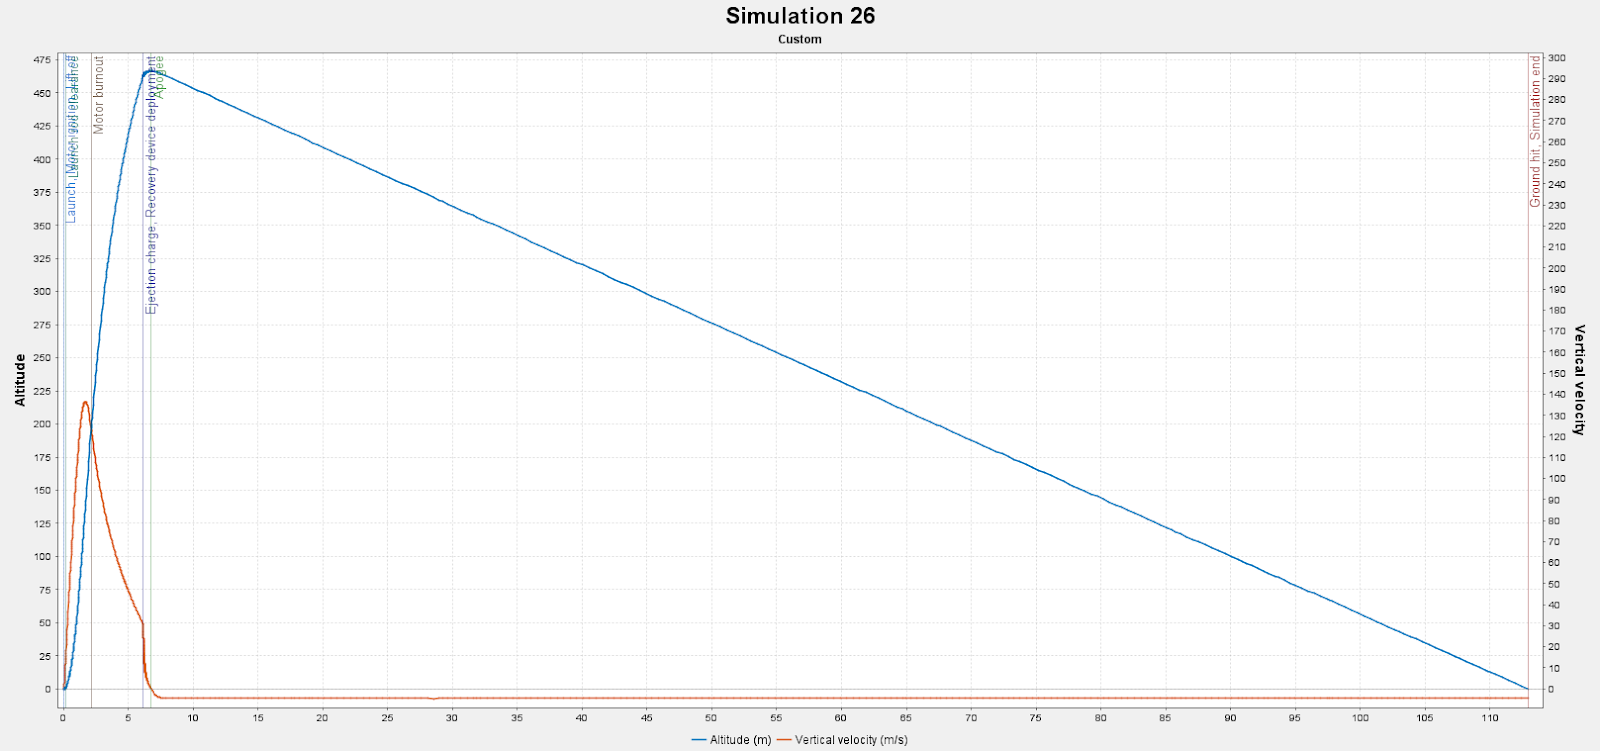
\includegraphics[width=0.9\linewidth]{sim26}
\caption{}
\end{figure}

\begin{figure}[H]
\centering
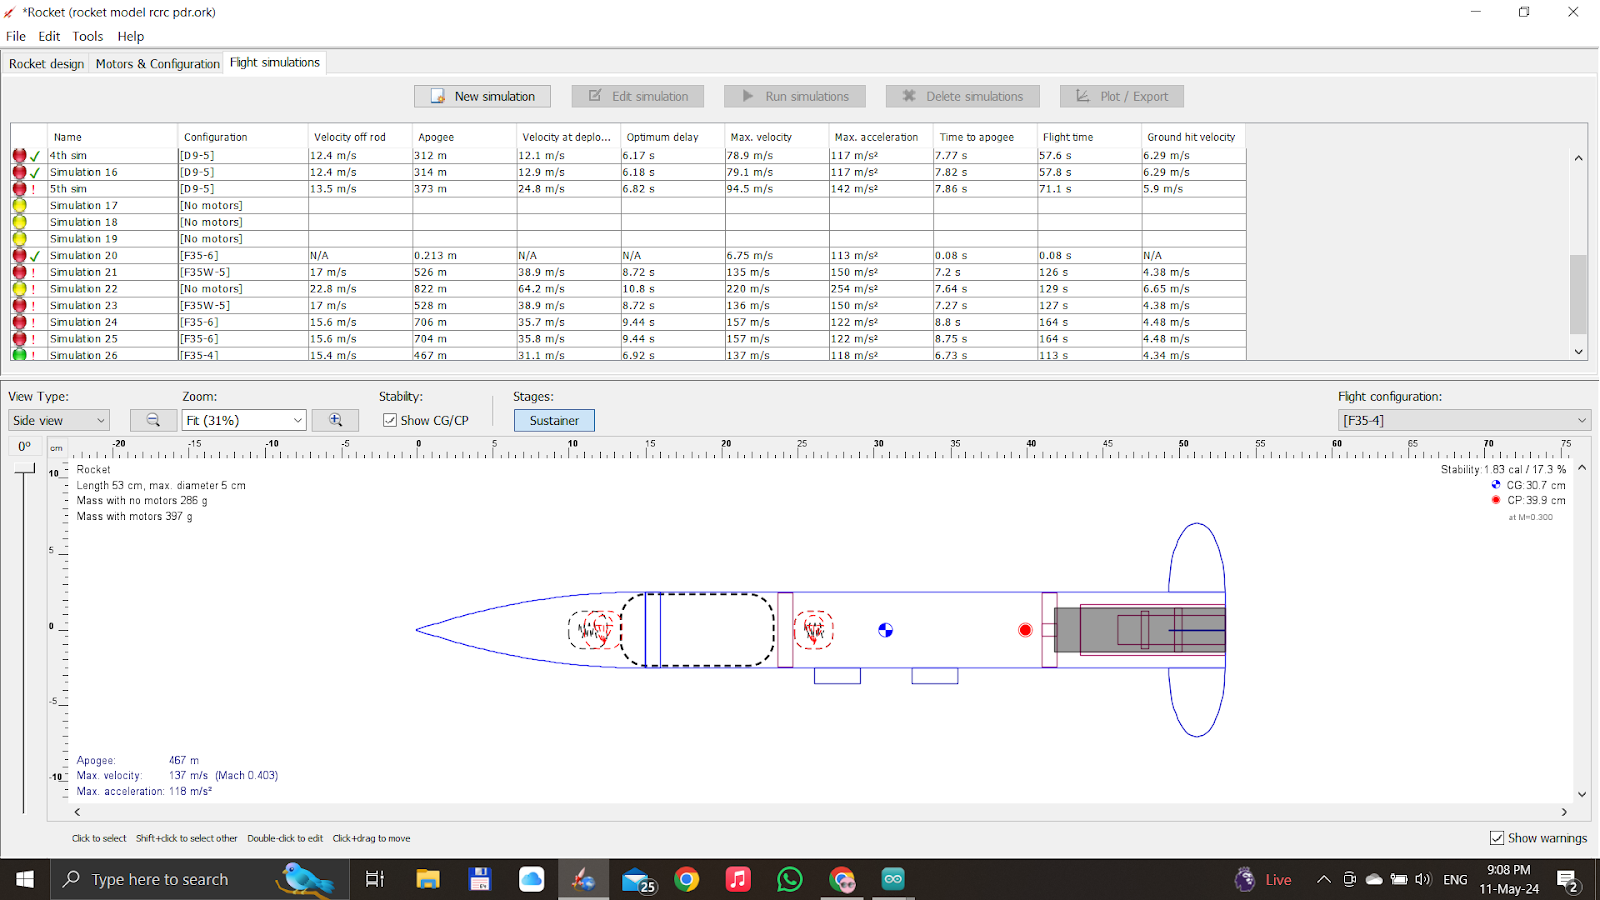
\includegraphics[width=0.9\linewidth]{rocketfin}
\caption{}
\end{figure}

\paragraph{Explanation}

The nose cone has the shape of a tangent ogive in order to be as aerodynamic as possible, thereby reducing air resistance. To ensure the stability of our rocket model, we might opt to add an extra weight in the cone, if the payload module doesn’t turn out to be heavy enough. The body tube will be made out of cardboard because we want to use a lightweight material that can also withstand the stress of launch and flight with high durability. The parachutes will be made out of Polyethylene, given that it is very thin, but resistant to shock and high forces, while the lines will be from braided nylon, and it will be tethered to the rocket model via an elastic shock cord. The bulkhead and engine block will be made of PLA, given that they need to withstand high shock forces. The inner tube will be from PLA, covering the motor, whereas the centering rings and launch lugs will be resistant enough to be made from cardboard, given its structural properties.

\subsubsection{Electrical design}

In this chapter we will present the exact details about the electrical design of the payload, including all the necessary components (controller and sensors) and how they will be connected. The power consumption of all the equipment will also be calculated, so that the perfect battery can be chosen.

\paragraph{Electrical Interface}

The electrical interface has two main objectives: data collection and data transmission. The microcontroller used is an Arduino NANO, chosen for its convenient size and connectivity options. There is also an APC220 radio transmitter connected to the main board. All of this is powered by a 9V battery. There are 3 sensors connected to it:

\begin{itemize}
 \item MPU6050 (acceleration, orientation)
 \item NEO-6M (GPS)
 \item BMP085 (atmospheric pressure)
\end{itemize}

Additionally, there is also an APC220 radio transmitter connected to the main board. All of this is powered by a 9V battery. Below is a scheme describing how all of these components come together:

\begin{figure}[H]
\centering
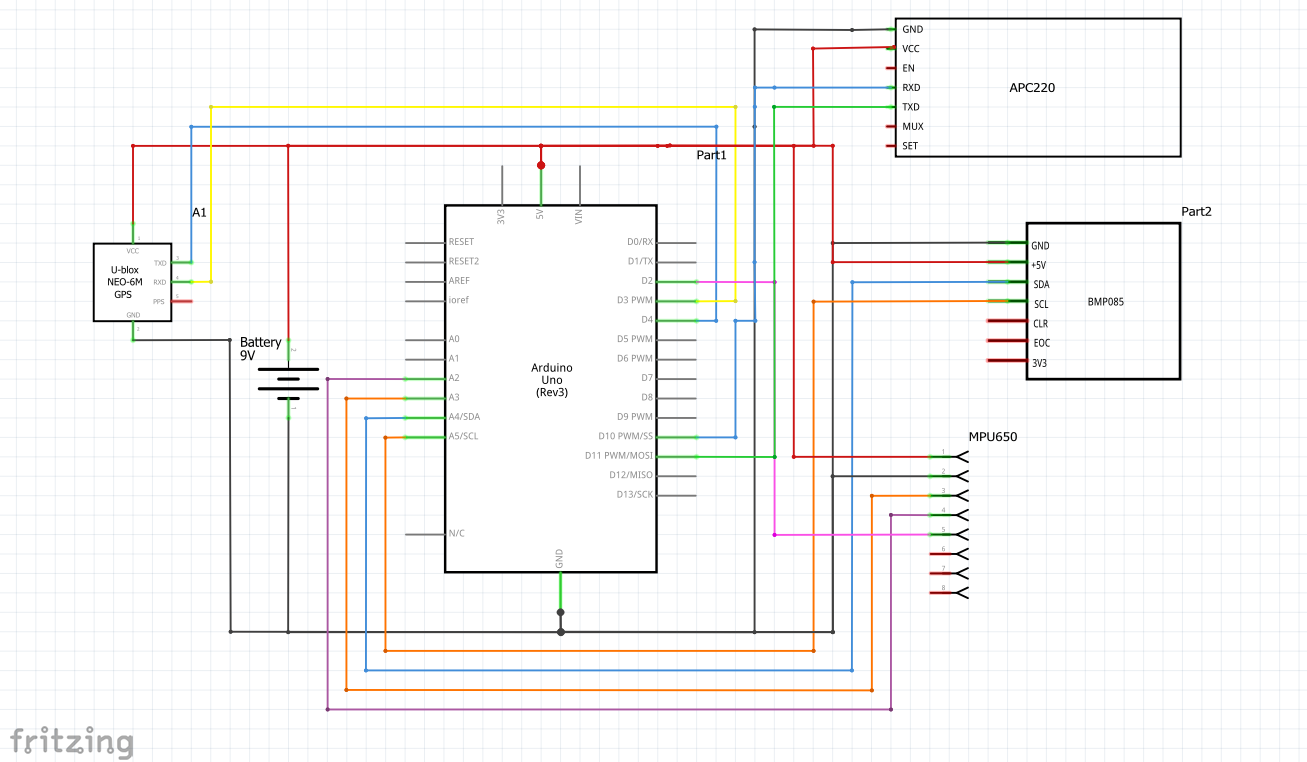
\includegraphics[width=0.9\linewidth]{elec_scheme_fin}
\caption{Electronic circuit}
\end{figure}

\paragraph{Radio Communication}

As we mentioned, we are using an APC220 for radio communication. This is for a couple of reasons, most importantly being its maximum transmission range: 1200 metres. We can also buy a second APC220 with a USB adaptor and connect it to our laptop, from the ground. We chose radio as our transmission method over wifi (via an ESP32), which has an inferior range of 200 metres. Internet transmission had the advantage of allowing us to use a more powerful protocol such as MQTT, a standard in IoT messaging. With our actual radio transmission, the CanSat computer sends a continuous stream of binary data, coupled with an error detection algorithm (Cyclic Redundancy Check), to ensure data integrity.

\paragraph{Power Consumption}

The power budget for the CanSat is as follows:

\begin{table}[H]
\centering
\begin{tabularx}{\textwidth}{|X|X|}
\hline
Component           & Power Consumption \\ \hline
Arduino NANO        & 1.5 W             \\
APC220              & 0.75 W            \\
MPU6050             & 0.004 W           \\
NEO-6M              & 0.07 W            \\
MicroSD             & 0.1 W              \\
BMP085              & 0.000005 W         \\ \hline
Total               & $ \sim $ 2.6 W     \\ \hline
\end{tabularx}
\end{table}

\subsubsection{Software design}

We are using C++17 as a programming language. The CanSat's software is highly object-oriented, as most components are abstracted. This allows us to define virtual interfaces for the hardware, which can be implemented for the real components but also for mock hardware, to enable testing on a computer. As a coding standard, we are using the JSF AV. The tasks are executed within a super loop.

\subsubsection{Software program flow}

The program flow can be seen in the following diagram:

\begin{figure}[H]
\centering
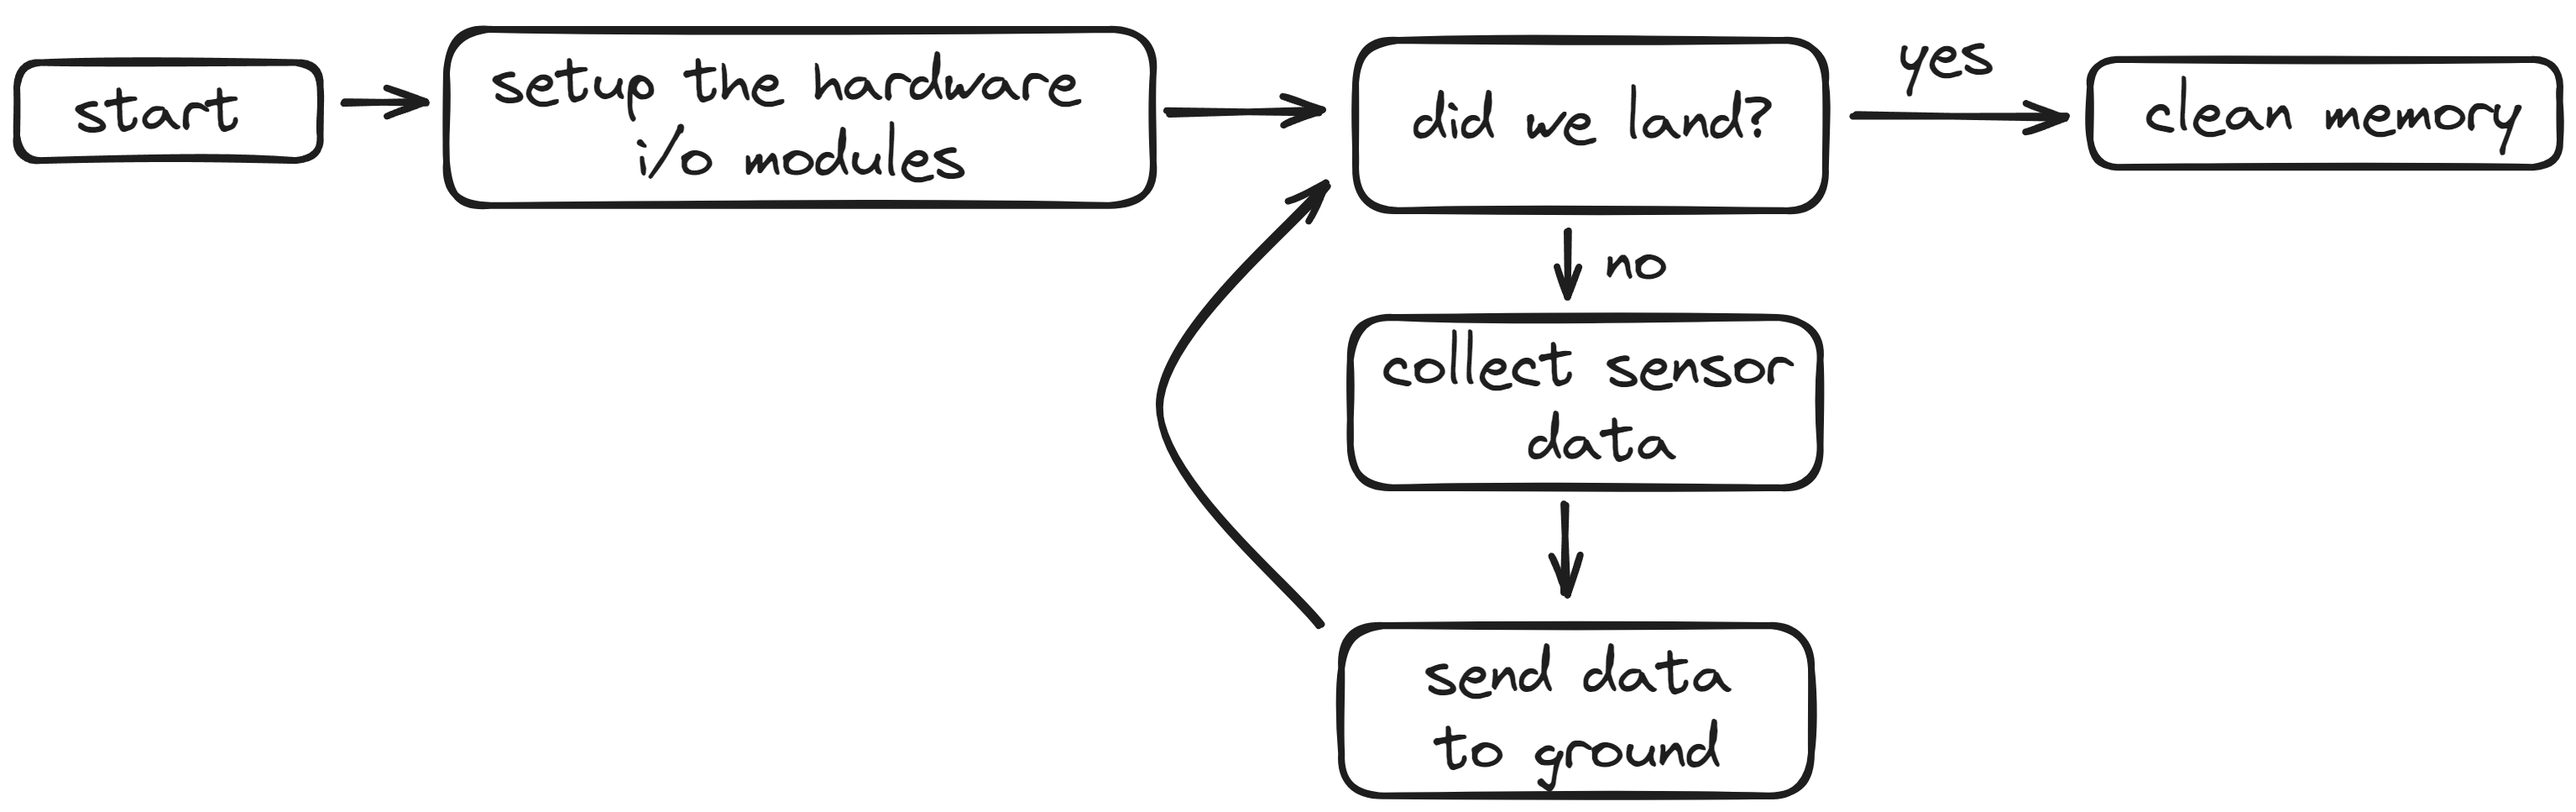
\includegraphics[width=0.9\linewidth]{flow_diagram}
\caption{Program flow}
\end{figure}

\subsubsection{Data Gathering and Storage}

To reduce complexity and costs, the CanSat doesn't store any long-term data. Instead, everything is transmitted to the ground station, where it's being processed and stored. The data is collected from the sensors, and sent via radio in a stream of binary data. We are using the Cyclic redundancy check (CRC) algorithm for error detection.To correct errors, the receiver (the ground station) has to send back an acknowledgement (ACK) or a negative acknowledgement (NACK). This process might add complexity, by requiring communication between the two devices. However an algorithm such as Forward error correction, which basically sends duplicate packets to correct any errors, adds too much garbage data and we need data fast to account for the entire duration of the mission, we can't afford any lag in our live data stream.

\subsubsection{Development Environment}

We are using an Arduino NANO as a microcontroller, which is powered by an ATmega328P microchip. To develop for this hardware, we are using the AVR toolchain. The code is written in C++17 and compiled with the avr-g++ compiler, and it's uploaded to the microcontroller using the avrdude command line tool. As a build tool, we are using GNU Make (makefiles).

\subsubsection{Recovery system}

Our rocket model will use a parachute with the diameter 417 mm for the recovery of the body tube and one with the diameter 217 mm for the recovery of the payload. As the motor runs out of fuel, the rocket reaches its apogee, and, after the 4 second delay, the loose black powder in the motors will build pressure inside the body tube, pushing the nose cone out, since the shoulder will intentionally not be very tight, to allow the safe deployment of our payload and the two parachutes.

\subsubsection{Ground support equipment}

The group equipment for the CanSat mission is composed of a laptop, with an APC220 radio receiver connected to it via a USB-C adaptor. The antenna is used to transmit and receive the data signals. The ground device has to respond with an acknowledgment (ACK) packet if the CRC checksum matches, so the CanSat knows there aren’t any errors in the transmitted data and can move on sending more packets. Otherwise, if the checksum doesn’t match, the receiver will reply with a negative acknowledgement (NACK) and the CanSat will send that packet again, hopefully without the same errors. More about the ground support device in the data analysis chapter. 